\paragraph{Scenarios}
    \begin{enumerate}
        \item Johnny is a model citizen of Milan and he is really caring about parking violations, because they are really frequent in his neighbourhood. When he sees a violation, he opens the SafeStreets app on his smartphone and reports it with just few clicks. All he needs to do is to take a photo of the violation where the license plate is clearly visible and confirm if the system detected it correctly or not, if not he inserts the license plate manually in the field that appears after the confirmation. Position is automatically detected from the GPS because he allowed the app to access it. Finally, to send the report to SafeStreets he just needs to confirm by clicking the done button.
        
        \item Giuseppe is a righteous citizen and recently has heard about SafeStreets but never used it. One day, he finds a double-parked car right in front of his, so he is not able to get his car out. After waiting some minutes hoping for the owner of the double-parked car to arrive without success, Giuseppe remembers about SafeStreets and decides to use it for the first time. He registers and logs in the app, then he uploads a photo of the car of the transgressor and sends the report. While still waiting, he checks whether his report has been validated by some authorities and sees that after 10 minutes it has been validated, so he now knows that the authorities will take action about it.
        
        \item George is a tourist who has just arrived in Rome, and plans to stay there for a week. When he goes out touring the city with the car he rented for the entire week, he uses SafeStreets to check where the most violation afflicted areas of the city are to avoid areas which can lead to a terrible experience in parking his vehicle. So he opens the SafeStreets app and enters the analyze data tab, selecting Rome as the city and a year time as time interval. George now knows where he should park his car and can have a great experience in Rome.
    \end{enumerate}
\textbf{Use cases}
\begin{figure}[H]
	\centering
    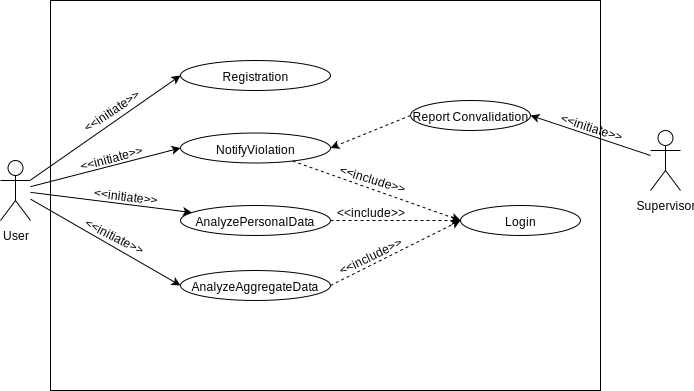
\includegraphics[width=\textwidth]{UML/UseCaseUser}
\end{figure}	



\begin{tabular}{|p{3.1cm}|p{11.6cm}|}
\hline
Name & Registration\\
\hline
Actors & Citizen\\
\hline
Entry Condition & The citizen opens the app and has no valid account.\\
\hline
Event flow & \begin{enumerate}
				\item The citizen inserts his last name.
				\item The citizen inserts his first name.
				\item The citizen inserts his birthday.
                \item The citizen inserts his email.
                \item The citizen inserts the desired password.
                \item The citizen confirms his password.
                \item The citizen agrees to the use of his personal data and of his submitted violation reports for analysis purposes.
            \end{enumerate}\\
\hline
Exit condition & The registration is successful and the citizen is redirected to login form.\\
\hline
Exception & Email is already in use or confirm password field content diverge from password, in this case the citizen is alerted with a proper message on screen and asked to correct the data.\\
\hline
\end{tabular}

\vskip 0.2in
\begin{tabular}{|p{3.1cm}|p{11.6cm}|}
\hline
Name & Login\\
\hline
Actors & Citizen\\
\hline
Entry Condition & The citizen opens the app.\\
\hline
Event flow & \begin{enumerate}
                \item The citizen inserts his email.
                \item The citizen inserts his password.
                \item The citizen press the login button.
            \end{enumerate}\\
\hline
Exit condition & The citizen is authenticated and login is successful.\\
\hline
Exception & Email or password are invalid, "invalid credentials" message is displayed and the citizen needs to insert credentials again.\\
\hline
\end{tabular}

\vskip 0.2in
\begin{tabular}{|p{3.1cm}|p{11.6cm}|}
\hline
Name & Report violation\\
\hline
Actors & Citizen\\
\hline
Entry Condition & Violation detection.\\
\hline
Event flow & \begin{enumerate}
                \item The citizen selects the "report a traffic violation" tab if not already selected.
                \item The citizen takes and uploads one or more photos of the violation.
                \item The citizen confirms that the license plate is correctly recognized by the app, if not he/she inserts it manually in the appropriate field.
                \item The citizen selects the type of violation.
                \item The citizen optionally inserts a short description of the violation in the description field.
                \item The citizen confirms the violation report clicking on the "Done" button.
                \item The system stores the information and completes it with suitable metadata.
                \item The system sends a notification to the citizen about the success of the operation.
            \end{enumerate}\\
\hline
Exit condition & The violation report is correctly stored.\\
\hline
Exception & the system detects missing information and rejects the report, then asks the citizen for missing data.\\
\hline
\end{tabular}

\vskip 0.2in
\begin{tabular}{|p{3.1cm}|p{11.6cm}|}
\hline
Name & Analyze aggregate data\\
\hline
Actors & Citizen\\
\hline
Entry Condition & The citizen wants to know some information about the reported violations.\\
\hline
Event flow & \begin{enumerate}
                \item The citizen selects the "analyze data" tab.
                \item The citizen selects the topic he/she is interested about.
                \item The citizen may select an appropriate filter for his search.
                \item The citizen selects the data of interest.
                \item The system provides the data to be visualized according to the actor's authorization level.
                \item The citizen visualizes the data.
            \end{enumerate}\\
\hline
Exit condition & The Actor finishes to analyze the data.\\
\hline
\end{tabular}

\vskip 0.2in
\begin{tabular}{|p{3.1cm}|p{11.6cm}|}
	\hline
	Name & Check personal reports\\
	\hline
	Actors & Citizen\\
	\hline
	Entry Condition & The citizen opens the app, desiring to check the reports he sent in the past.\\
	\hline
	Event flow & \begin{enumerate}
		\item The citizen selects the "analyze personal reports" tab.
		\item The system displays a list of all reports done by the citizen.
		\item The citizen clicks on a report to see its details.
		\item The citizen clicks the return button, going back to the list of reports.
		\item The citizen can repeat the last two steps as many times as he pleases, to check other reports.
	\end{enumerate}\\
	\hline
	Exit condition & The citizen closes the reports list after he doesn't need to visualize them anymore.\\
	\hline
\end{tabular}

% sequence diagrams
\newpage
\textbf{Sequence diagrams}
\begin{figure}[H]
	\centering
	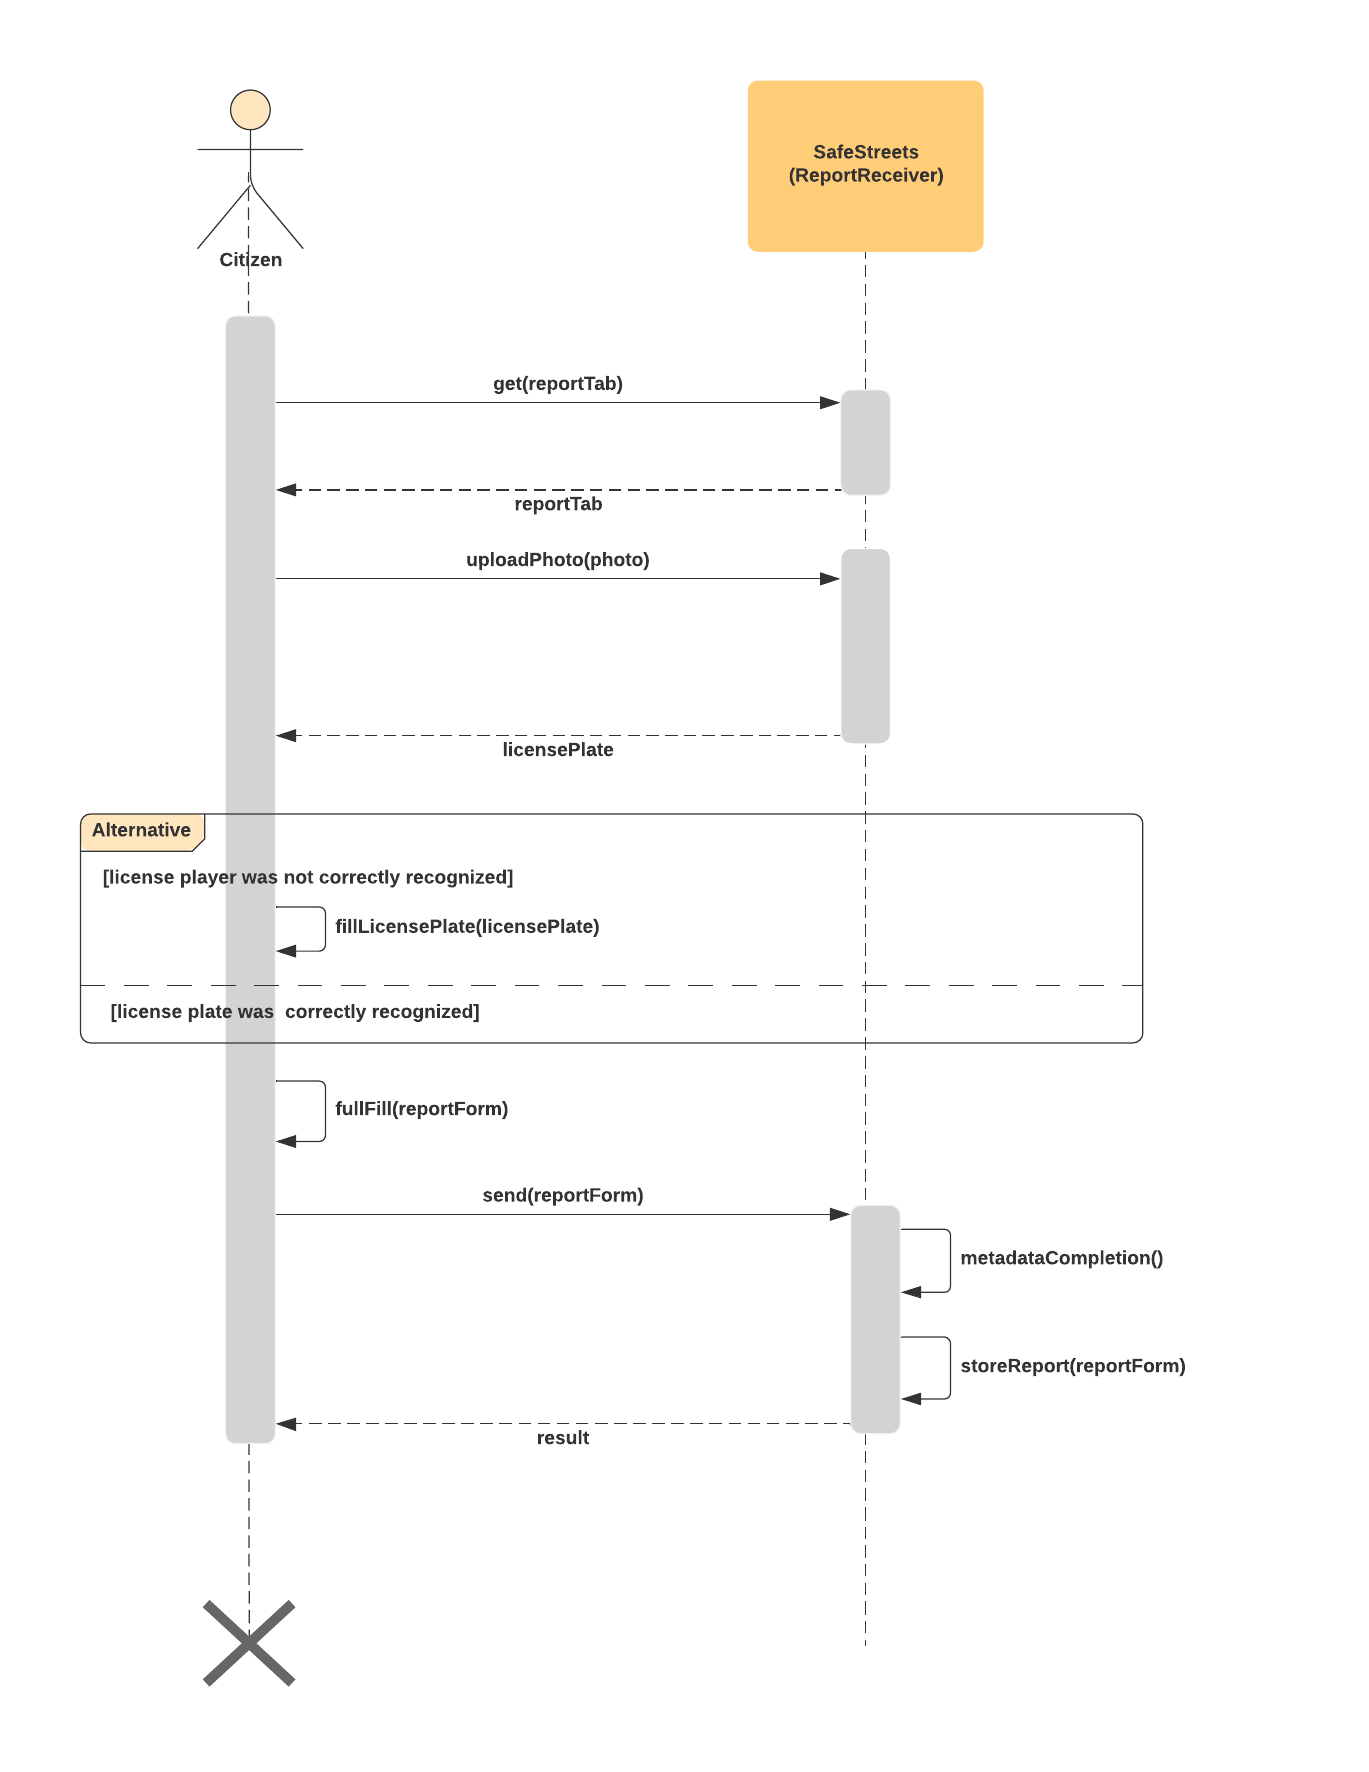
\includegraphics[width=\linewidth]{Images/UML/NotifyViolationUseCase}
	\caption{Report violation use case.}
\end{figure}
\begin{figure}[H]
	\centering
	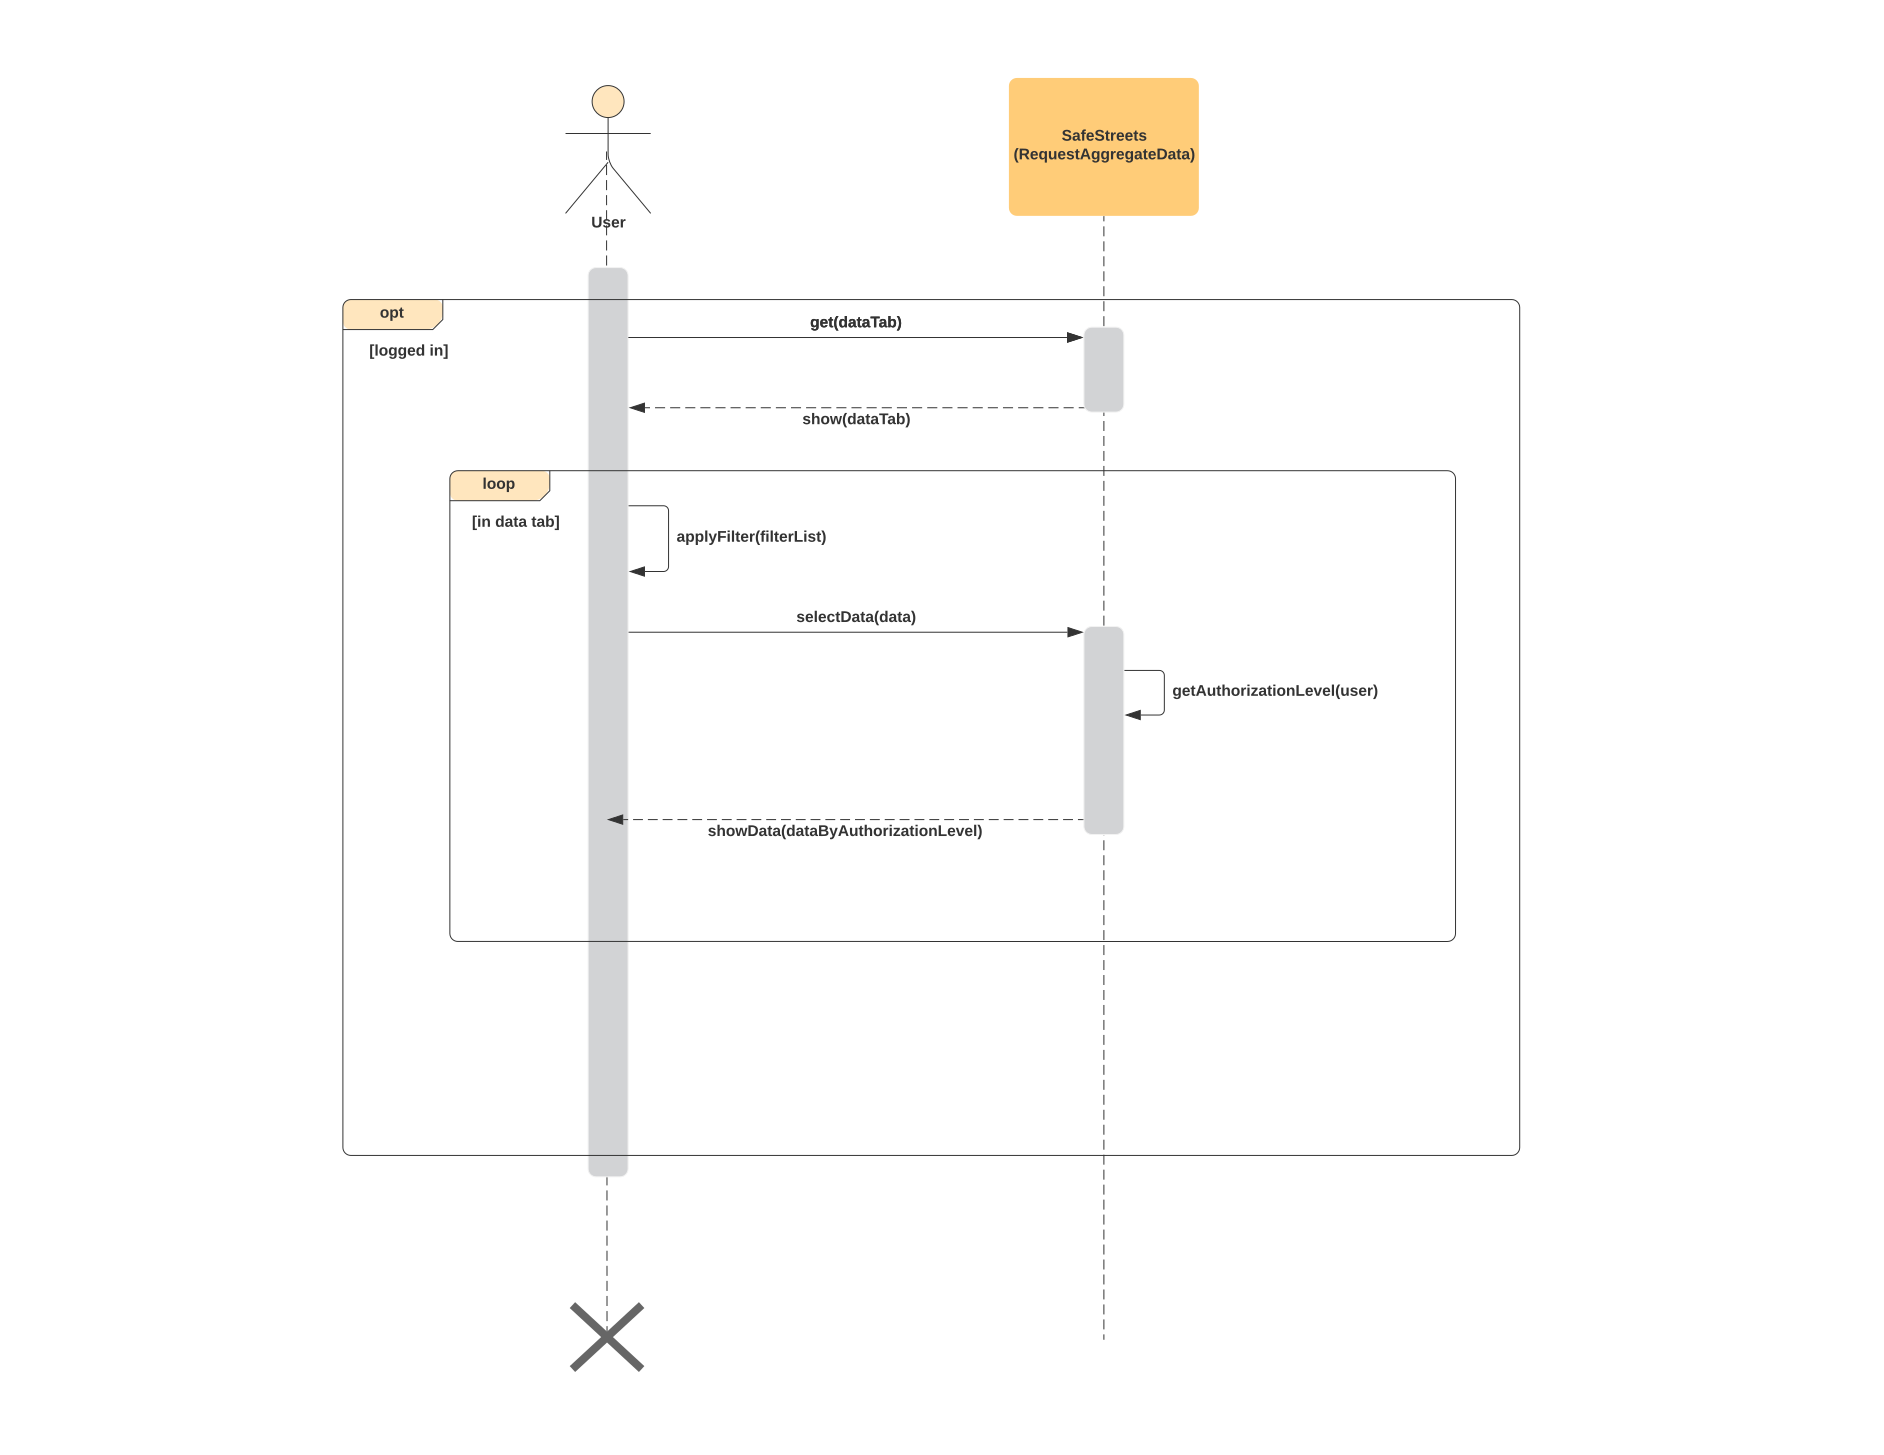
\includegraphics[width=\linewidth]{Images/UML/AnalyzeDataUseCase}
	\caption{Analyze aggregate data use case.}
\end{figure}
